\documentclass[11pt]{article}

% parameters are fairly self-explanatory here, thankfully
\usepackage[width=7in,height=9.5in,top=0.75in,centering]{geometry}

% for math-ing
\usepackage{amsmath}
\usepackage{amssymb}


%%%%%% tables %%%%%%%%

\usepackage{array}
\renewcommand{\arraystretch}{1.5}
\setlength{\tabcolsep}{8pt}

%%%%%% plotting %%%%%%

\usepackage[dvipsnames]{xcolor}
\usepackage{tikz}
\usepackage{pgfplots}

\pgfplotsset{every axis/.append style={
                    axis x line=middle,    % put the x axis in the middle
                    axis y line=middle,    % put the y axis in the middle
                    axis line style={<->,color=black}, % arrows on the axis
                    xlabel={$x$},          % default put x on x-axis
                    ylabel={$y$},          % default put y on y-axis
            }}
            
 \pgfplotsset{compat=1.14} % sometimes, everything falls apart without this
 
 %\usepgfplotslibrary{fillbetween} %for shading between curves

%%%%%% commands %%%%%%

% exam heading; course name is first argument, exam information is second argument
\newcommand{\Heading}[2]{
    \fbox{
        {\Large\textbf{#1}}
        }
    \hfill
    \fbox{
        \begin{minipage}{0.2\textwidth}
            \begin{center}
            \textbf{#2}
            \end{center}
        \end{minipage}
    }
    \par\vspace{0.1in}}

% for being lazy while beautifying integrals
\newcommand{\dint}{\displaystyle\int}

% for being lazy while beautifying limits
\newcommand{\dlim}{\displaystyle\lim}

%%%%%% stuff %%%%%%

\usepackage{fancyhdr}

%\setcounter{page}{0} % first page is page 0

\parindent0pt % no indent

\fboxsep=0.25cm % little space in fbox border

%%%%%% BEGIN! %%%%%%%

\begin{document}

\pagestyle{fancy}

% record goals here to create sense of transparency

\fancyhead[l]{%
  \ifcase\value{page}
  % empty test for page = 0
  \or {}% 
  \or
  \or {\bf\color{ProcessBlue} F1: Lines \& Slope}% page=1
  \or {\bf\color{RoyalBlue} L1: Limits and Continuity}% page = 2
  \or {\bf\color{RoyalBlue} L2: Evaluating Limits Using Continuity and Forms}% page = 3
  \or {\bf\color{ForestGreen} D1: Meaning of a Derivative}% page = 4
  \or {\bf\color{ProcessBlue} F2: Exponential and Logarithmic Functions}% page = 5
  \or {\bf\color{ForestGreen} D2: Compute Derivatives}% page = 6
  \or {\bf\color{ForestGreen} D3: Derivatives of Basic Functions}% page = 7
  \or {\bf\color{RedOrange} A1: Derivatives and Graphing}% page = 8
  \or
  \else
  % Empty chead here!
  \fi
}

\thispagestyle{empty} % don't display that this is page 0

\Heading{MATH 1190/1210 Survey of Calculus I}{Quiz ?\\Learning Target A2\\Fall 2025}

\vspace{0.1in}

\textbf{Name} \hrulefill \, \begin{minipage}{0.16\textwidth}\begin{center}\textbf{UVA ID\\ (e.g. hdj4nd)} \end{center}\end{minipage}\hrulefill\\




%%%%%%%%%%%%%%%%%%%%%%%%%%%%%%%%%%%%%%%%%%%%%%%%%%%%%
%%%%%%%%%%% BEGIN PROBLEM A1 %%%%%%%%%%%%%%%%%%%%%%%%
%%%%%%%%%%%%%%%%%%%%%%%%%%%%%%%%%%%%%%%%%%%%%%%%%%%%%

Let $f(x)=\dfrac13x^3-x^2+\dfrac13$.
\begin{enumerate}
\item[(a)] Find the critical numbers of $f$.

    \vfill
\item[(b)] Classify all local extrema of $f$. 
\vfill
\item[(c)] Find absolute extrema on $[0,1]$
\vfill
\end{enumerate}

%%%%%%%%%%%%%%%%%%%%%%%%%%%%%%%%%%%%%%%%%%%%%%%%%%%%%
%%%%%%%%%%% END PROBLEM A1 %%%%%%%%%%%%%%%%%%%%%%%%%%
%%%%%%%%%%%%%%%%%%%%%%%%%%%%%%%%%%%%%%%%%%%%%%%%%%%%%


\end{document}
\item ({\bf\color{RedOrange}M1: Local Maxima \& Minima})\\[0.1in]
%


\soln{First and foremost, we note that the domain of $f(x)$ is the whole real line $\left(-\infty, +\infty\right)$ because $f(x)$ is a polynomial, thus everywhere defined, continuous, and differentiable as many times as one fancies to differentiate it. This domain computation is inescapable, for a critical number of $f(x)$ is required to lie in the domain of $f(x)$, so we need to have computed the domain of $f(x)$ in advance to tell which numbers can and cannot be critical numbers of $f(x)$. \\ \\
Now, we may safely proceed with computing $f'(x)$ and detecting all numbers where $f'(x)$ is equal to zero or is undefined, ideally knowing in advance that the latter will not be the case at any real number because the polynomial $f(x)$ is everywhere differentiable, as we discussed:
$$f'(x)=x^{2}-2x$$
Indeed, as we knew in advance, $f'(x)$ is defined everywhere. To detect all numbers where $f'(x)$ vanishes - that is, all numbers where $f'(x)$ is equal to zero - we fully factor $f'(x)$ as follows:
$$f'(x)=x^{2}-2x=x\left(x-2\right)$$
and we read that $f'(x)$ vanishes precisely at $x=0$ and at $x=2$, both of which lie in the domain $\left(-\infty, +\infty\right)$ of the polynomial $f(x)$. Hence, \fbox{the critical numbers of $f(x)$ are $x=0$ and $x=2$}.}

\item[(b)] Use the First Derivative Test to find all local extrema of $f$. Your work must show how the conditions of the First Derivative Test are or are not satisfied to receive full credit.

\soln{Having fully factored the first derivative $f'(x)$ of the polynomial $f(x)$ as follows:
$$f'(x)=x\left(x-2\right)$$
we are in the advantageous position to compute the sign chart for $f'(x)$ as follows:

\begin{center}

\begin{tikzpicture}
\tkzTabInit[lgt=2,espcl=2,deltacl=0]
  { /.8, $x$ /.8, $x-2$ /.8, $f'(x)$ /.8}
  {,$0$,$2$,} % four main references
\tkzTabLine {,-,z,+,t,+,} % seven denotations
\tkzTabLine {,-,t,-,z,+,}
\tkzTabLine {,+,z,-,z,+,}
\end{tikzpicture}

\end{center}
The above sign chart combined with the first derivative test for local extrema informs us that:

\begin{enumerate}
    \item \fbox{the critical number $x=0$ is a local maximum with local maximum value $f(0)=\dfrac{1}{3}$} \linebreak because the sign of the first derivative $f'(x)$ of the polynomial $f(x)$ changes from $+$ to $-$ at the critical number $x=0$ of $f(x)$, and that
    \item \fbox{the critical number $x=2$ is a local minimum with local minimum value $f(2)=-1$} \linebreak because the sign of the first derivative $f'(x)$ of the polynomial $f(x)$ changes from $-$ to $+$ at the critical number $x=2$ of $f(x)$.
\end{enumerate}
\noindent Since the local extrema of a function are only attained at critical numbers of said function, our above list of local extrema of $f(x)$ is exhaustive, as required. Thus, this concludes our work.
}

\end{enumerate}